\subsection{Timing Performance Results from Calorimeter with SiPM Readout}
\label{sec:beamtiming}

Four different SiPMs are used to read out the four light fibers. As they each have
different gain and light collection efficiency, the signal amplitude response varies
for the four different channels. In Figure~\ref{TimeResolution} we show the time 
resolution of the four individual fibers as a function of their respective signal 
amplitudes. We observe that the time resolution improves as the amplitude of the pulses 
increases. The best time resolution per fibre is around $60$~ps for all of the channels, 
but the amplitude at which this performance is achieved varies.
Another important observation is that the time resolution measured from
the DSB-doped WLS fibers fall on the same curve as the time resolution measured from
the quartz capillaries. We conclude that the method of light extraction
impacts the time resolution only through its effect on the signal amplitude, and
no additional time jitter is introduced. 

%
\begin{figure}[htb]
%\hspace*{-0.3cm}
%\begin{minipage}[b]{22pc}
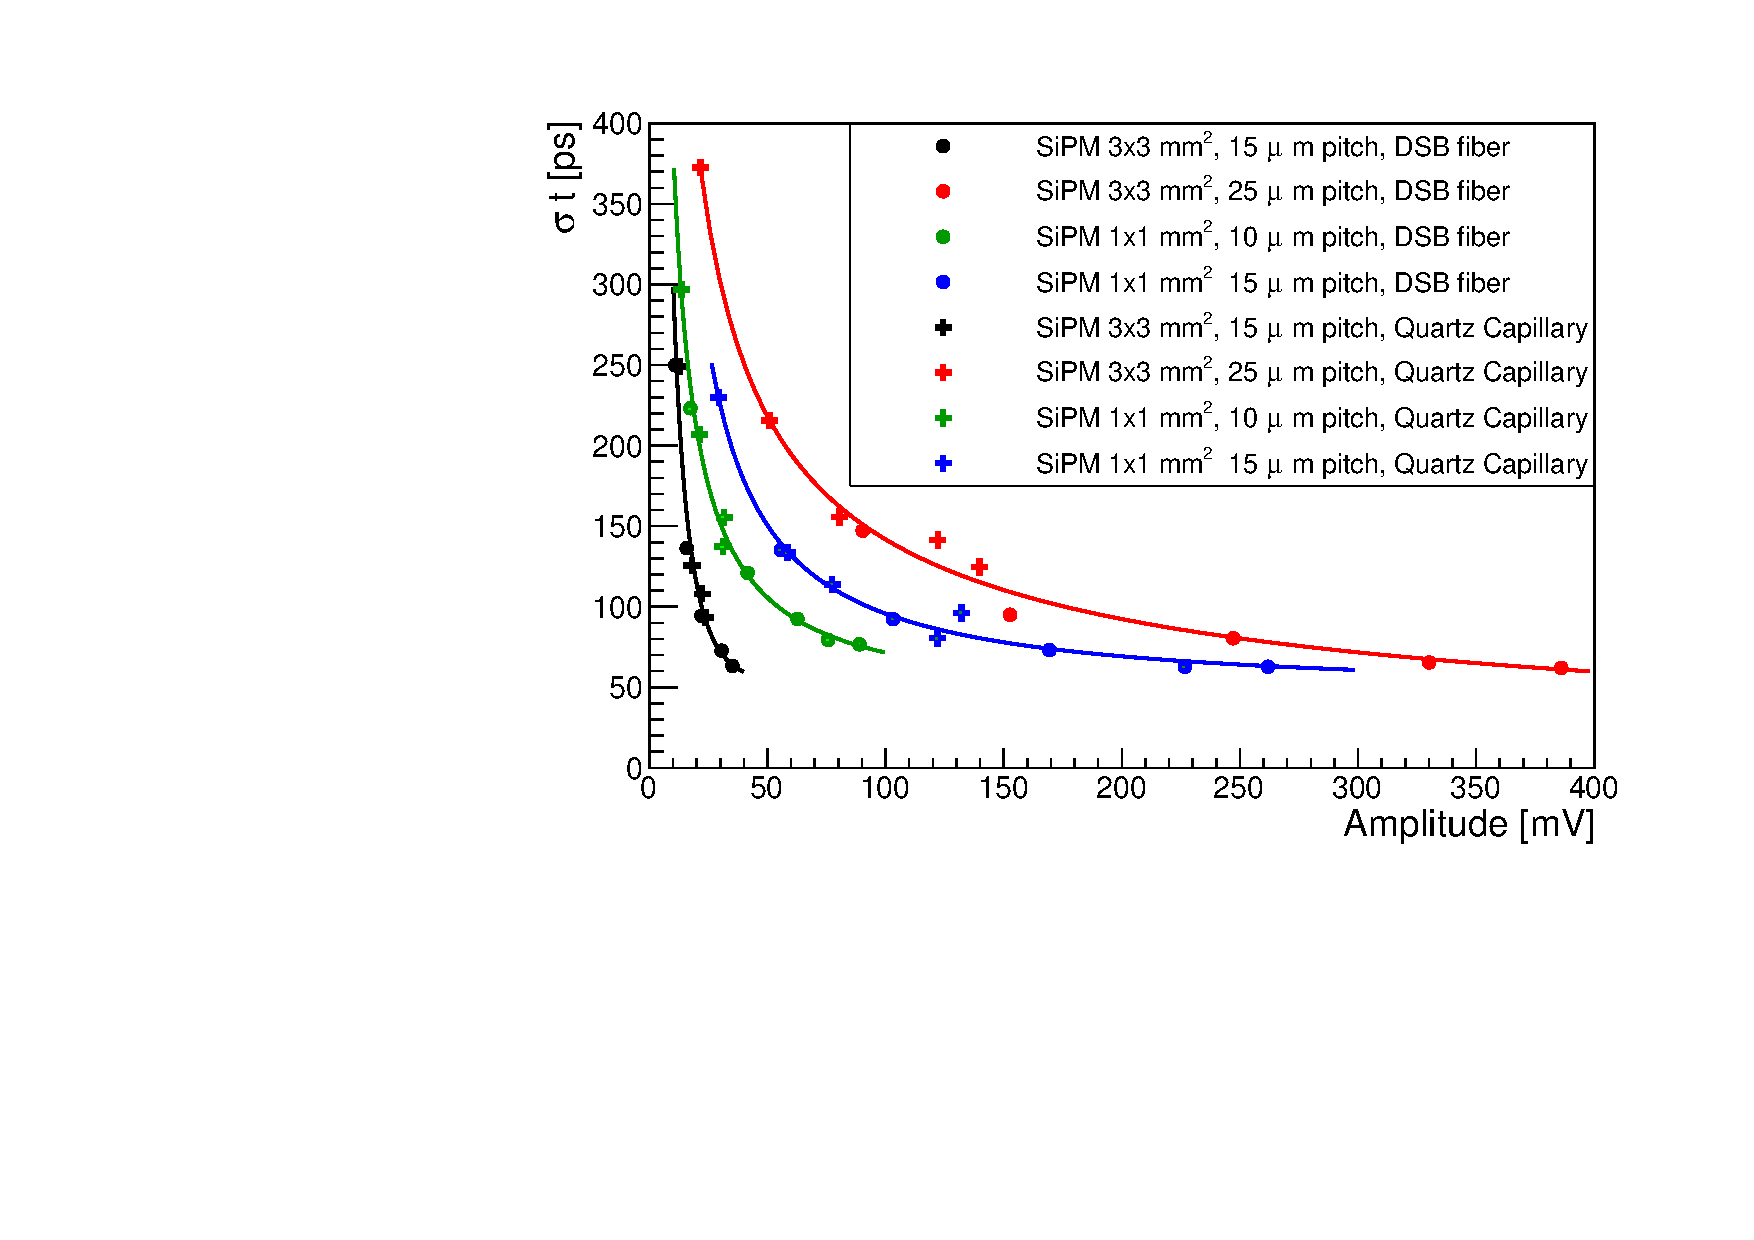
\includegraphics[width=0.99\textwidth]{figures/ShashlikTimeResolution.pdf}
%\end{minipage}
%\begin{minipage}[b]{14pc}
\caption{\label{TimeResolution} Time resolution achieved with the calorimeter cell using the signal of each 
of the  SiPMs individually. The data for each SiPM consists of two sets, one with the DSB WLS plastic fiber shown as 
dots and one with the capillaries with a liquid DSB based WLS shown as squares. }
%\end{minipage}
%\hspace*{-0.3cm}
\end{figure}
%


As the time measurement precision depends on the rise time of the pulse we also
measure the time resolution as a function of the rise time for signals observed 
in the calorimeter cell shown in Figure~\ref{RiseTime}. The risetime of these signals 
are driven by the time constants of the wave length shifter as 
demonstrated in reference~\cite{lysotiming}. We observe that the risetime
ranges between X ns and Y ns and that the time resolution improves as the 
risetime of the signals decrease. 

%
\begin{figure}[htb]
%\hspace*{-0.3cm}
%\begin{minipage}[b]{22pc}
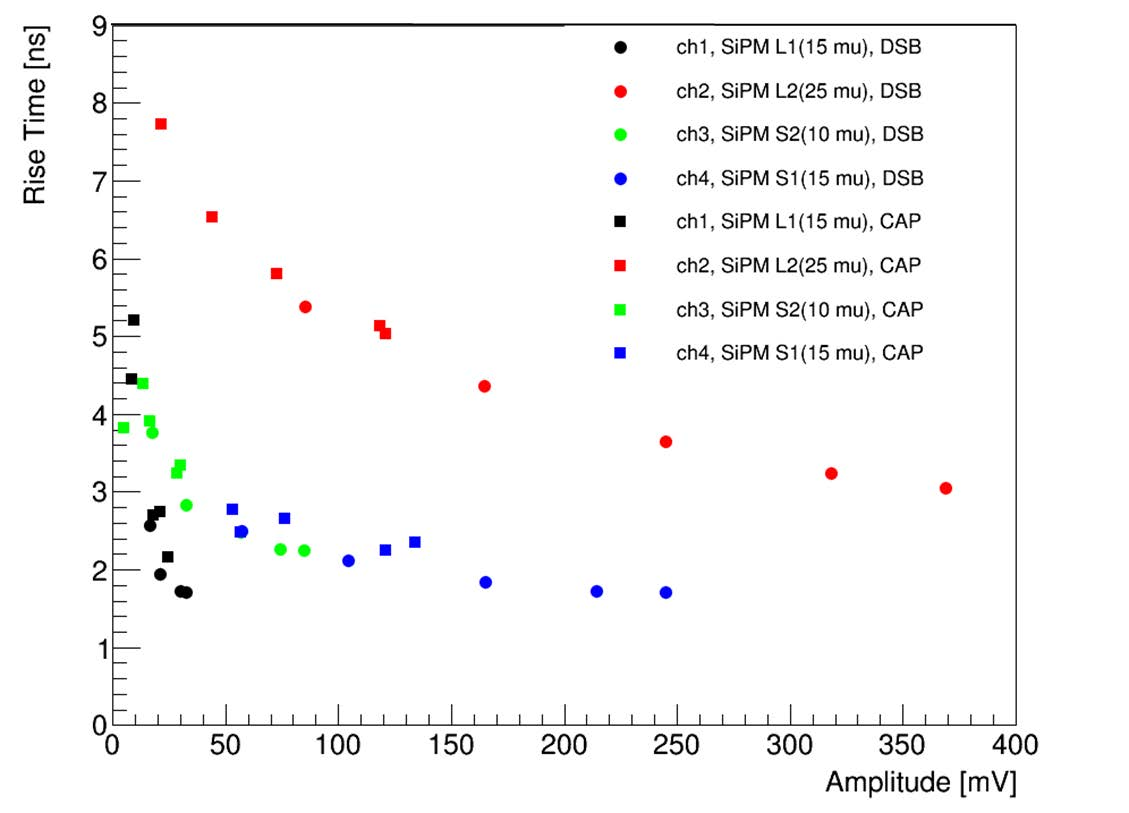
\includegraphics[width=0.99\textwidth]{RiseTime.pdf}
%\end{minipage}
%\begin{minipage}[b]{14pc}
\caption{\label{RiseTime}Time resolution is measured as a function of the risetime
for the four different SiPMs. The data recorded with the DSB WLS fibers and the
quartz capillaries are distinguished as dots and squares. }
%\end{minipage}
%\hspace*{-0.3cm}
\end{figure}
%


We show the time resolution measured as a function of the beam energy for
data read out by DSB WLS fibers and quartz capillaries in 
Figure~\ref{TimeResolutionVsEnergy}. Finally, by combining the measured timestamp
from all four SiPM channels, we can significantly improve the time resolution.
The results for the DSB WLS fibers and the quartz capillaries are shown in
Fig~\ref{TimeResolutionCombined} and demonstrate that we can achieve time resolution
below $50$~ps for high energy electromagnetic showers.

%
\begin{figure}[htb]
%\hspace*{-0.3cm}
%\begin{minipage}[b]{22pc}
\includegraphics[width=0.99\textwidth]{figures/TimeResolutionVsBeamEnergy_DSB.pdf}
\includegraphics[width=0.99\textwidth]{figures/TimeResolutionVsBeamEnergy_Capillary.pdf}
%\end{minipage}
%\begin{minipage}[b]{14pc}
\caption{\label{TimeResolutionVsEnergy} Time resolution measured in the sampling calorimeter cell using the signal of each 
of the SiPMs individually as a function of the beam energy. The data taken using DSB WLS fibers are shown on
the left and the data taken using quartz capillaries are shown on the right}
%\end{minipage}
%\hspace*{-0.3cm}
\end{figure}
%

%
\begin{figure}[htb]
%\hspace*{-0.3cm}
%\begin{minipage}[b]{22pc}
\includegraphics[width=0.99\textwidth]{figures/TimeResolutionCombinedChannelsVsBeamEnergy.pdf}
%\end{minipage}
%\begin{minipage}[b]{14pc}
\caption{\label{TimeResolutionCombined}  Time resolution measured in the sampling calorimeter cell combining signals from all four  
SiPMs is shown as a function of the beam energy.  The data recorded with the DSB WLS fibers and the
quartz capillaries are distinguished as dots and squares.}
%\end{minipage}
%\hspace*{-0.3cm}
\end{figure}
%


The light extraction efficiency of capillaries with liquid WLS remains
sufficiently high for dose rates of $100$~Mrad and beyond and for fluences of
$10^{14}$~protons/$\mathrm{cm}^{2}$ and beyond~\cite{shashlik2}. This result
demonstrates the feasibility of achieving good time resolution using a sampling
calorimeter based on LYSO which can survive in dense hadronic collision environments.
The energy resolution performance of the LYSO-tungsten cell is not limited by
photo-statistics but is rather limited by the sampling fraction. Therefore, the timing
performance could be improved by increasing the signal size, for example by 
using larger diameter capillaries.\\ 

